\documentclass[]{report}
\usepackage[table,xcdraw]{xcolor}
\usepackage[Glenn]{fncychap}
\usepackage[T1]{fontenc}
\usepackage[francais]{babel}
\usepackage{fontspec}
\usepackage{wrapfig}
\usepackage{graphicx}
\usepackage[a4paper, width=175mm, top=25mm, bottom=25mm]{geometry}
\usepackage{parskip}
\usepackage{enumitem}
\usepackage{titlesec}
\usepackage{listings}
\usepackage{float}
\usepackage[final]{pdfpages}
\usepackage{tocbibind}
\usepackage{tocloft}
\usepackage{xpatch}
\usepackage{amsmath}
\usepackage{amsthm}
\usepackage{amsfonts}
\usepackage{graphics}
\usepackage{framed}
\usepackage{multirow}
\usepackage{graphicx}
\usepackage[utf8x]{inputenc}
\usepackage{mathtools}
\usepackage{amsmath}
\usepackage{tabularx}
\usepackage{tikz}
\usepackage{multirow}
\usepackage[noend]{algpseudocode}
\usepackage{tabularx}  % for tabularx


\lstset{
	literate=%
	{à}{{\'a}}1
	{í}{{\'i}}1
	{é}{{\'e}}1
	{è}{{\`e}}1
	{ý}{{\'y}}1
	{ú}{{\'u}}1
	{ó}{{\'o}}1
	{ě}{{\v{e}}}1
	{š}{{\v{s}}}1
	{č}{{\v{c}}}1
	{ř}{{\v{r}}}1
	{ž}{{\v{z}}}1
	{ď}{{\v{d}}}1
	{ť}{{\v{t}}}1
	{ň}{{\v{n}}}1
	{ů}{{\r{u}}}1
	{Á}{{\'A}}1
	{Í}{{\'I}}1
	{É}{{\'E}}1
	{Ý}{{\'Y}}1
	{Ú}{{\'U}}1
	{Ó}{{\'O}}1
	{Ě}{{\v{E}}}1
	{Š}{{\v{S}}}1
	{Č}{{\v{C}}}1
	{Ř}{{\v{R}}}1
	{Ž}{{\v{Z}}}1
	{Ď}{{\v{D}}}1
	{Ť}{{\v{T}}}1
	{Ň}{{\v{N}}}1
	{Ů}{{\r{U}}}1
}

\begin{document}


	\includepdf[pages=1]{Page_garde.pdf} 
	
	\tableofcontents

	\listoffigures

	
	\chapter{Introduction }
	\paragraph{}
	La théorie des possibilité offre de nombreux outils pour représenter des connaissances , et faire de l'inférence sur la ces bases de connaissances, parmi ces outils, nous allons étudier dans ce TP nous allons nous intéresser à la comparaison des performances de deux
	méthode d'inférence, par propagation et par inférence logique, nous allons tout d'abord introduire les outils utilisés, puis nous allons expliquer les étapes de transformation d'un graphe possibiliste en une base logique possibiliste, puis nous essayerons les deux algorithmes sur un ensemble de test, en paramétrant à chaque fois le volume de données en entrée(ces données sont générées aléatoirement).
	d'observations, parmis elles 
	\chapter{Réalisation}
	\section{Les outils utilisés}
	\subsection{Matlab-PNT}
	\paragraph{}
	Pour ce qui est de la représentation graphique, nous disposons d'un très bon outil, la PNT sous Matlab, nous pouvons donc l'utiliser pour concevoir nos réseaux, et appliquer des algorithme de propagation(basé sur le min par exemple), principalement, nous allons l'utiliser pour la comparaison entre des graphes avec peu(beaucoup) de noeud-connections
	et son équivalent en base possibiliste, pour faire la conversion l'outil Cygwin est nécessaire.
	\subsection{Cygwin}
	 Il faut savoir que pour transformer un graphe possibiliste en une base possibiliste, nous devons tout d'abord effectuer une conversion des relations entre les noeuds dans le modèle graphique en formules logique pondérées dans la base possibiliste.
	 \par 
	 Pour ce faire nous avons a disposition un algorithme de transformation ainsi qu'un solveur max-sat qui tournent sous un environnement Unix, d'où l'utilisation de l'outil Cygwin qui permet de simuler un tel environnemt dans Windows.
	 
	\section{Propagation de possibilité sur une évidence}
	\subsection{Utilisation du prod1vid.m}
	Le script \textbf{prod1vid.m} se charge en gros, de créer un DAG(Directed Acyclic Graph) de tester si c'est un Poly-arbre ou un graphe multi-connecté (test de présence de cycle), puis génère aléatoirement selon les paramètres nbr-nodes et nbr-parent-max une distribution de possibilité en respectant la contrainte $max(\pi(e_i)=1$.
	\par Nous avons  pris la peine de modifier le code pour le transformer en fonction qu'on pourra appeler depuis un autre script en passant les deux paramètres \textbf{nbr-nodes} et \textbf{nbr-parent-max}, cela pour automatiser le teste des instances.
	
	\section{Réglage automatique des paramètres}
	\subsection{Jeu de test}
	Différentes valeurs pour nb-node et diffèrent nb-parent-max ont été testées par le biais de notre mini script \textbf{test\_any.m}, le but est à chaque fois de fixer le nombre de parent, et faire varier le nombre de noeud, de ce fait nous jouons sur la nature(nb-parent < 2 donc poly-arbre) et la densité (nbr-parent>2 donc multi-connecté) du réseau, et à chaque fois nous récupérons le temps de propagation (éventuellement après construction de l'arbre de jonction dans le cas du multi-connecté), nous passons ensuite à l'exécution du convertisseur \textbf{passage.exe}, qui construit la base possibiliste correspondant au réseau généré ultérieurement.
	\subsection{Résultats}
	Pour résumer le travail effectué, nous avons dressé ces tableaux comparatifs, en fonction des nombres de parents max et du nombre de noeuds, comme demandé, nous avons réalisé les teste sur les 4 catégories suivantes : 
	\subsubsection{Poly-arbre}
	Pour s'assurer de la génération d'un poly-arbre, nous avons fixé le nombre maximum de parent à 1, nous avons ensuite fait varier le nombre de noeuds dans le réseau. Voici les résultats obtenues : 
	%POLYTREE
    \begin{table}[H]
    \resizebox{\textwidth}{!}{%
    \begin{tabular}{|c|c|c|c|c|}
    \hline
    \textbf{Nombre noeud} & \textbf{Nombre parent} & \textbf{degré de possibilité} & \textbf{Temps de propagation} & \textbf{Temps d'inférence} \\ \hline
    8                     & 1                      & 0.00091188                    & 0.010118                      & 0.03125                    \\ \hline
    10                    & 1                      & 0.36788                       & 0.012258                      & 0.03125                    \\ \hline
    12                    & 1                      & 0.00091188                    & 0.014352                      & 0.03125                    \\ \hline
    14                    & 1                      & 0.018316                      & 0.016613                      & 0.03125                    \\ \hline
    16                    & 1                      & 3.06E-07                      & 0.019468                      & 0.03125                    \\ \hline
    18                    & 1                      & 0.13534                       & 0.021925                      & 0.03125                    \\ \hline
    20                    & 1                      & 0.13534                       & 0.024707                      & 0.03125                    \\ \hline
    22                    & 1                      & 0.00091188                    & 0.027159                      & 0.046875                   \\ \hline
    24                    & 1                      & 1                             & 0.029406                      & 0.046875                   \\ \hline
    26                    & 1                      & 0.13534                       & 0.032944                      & 0.046875                   \\ \hline
    28                    & 1                      & 0.13534                       & 0.037111                      & 0.046875                   \\ \hline
    30                    & 1                      & 0.0024788                     & 0.039238                      & 0.046875                   \\ \hline
    32                    & 1                      & 1                             & 0.039181                      & 0.046875                   \\ \hline
    34                    & 1                      & 0.0024788                     & 0.042355                      & 0.046875                   \\ \hline
    36                    & 1                      & 1                             & 0.061121                      & 0.046875                   \\ \hline
    38                    & 1                      & 0.0024788                     & 0.052535                      & 0.03125                    \\ \hline
    40                    & 1                      & 1                             & 0.054939                      & 0.03125                    \\ \hline
    42                    & 1                      & 0.049787                      & 0.05315                       & 0.046875                   \\ \hline
    44                    & 1                      & 1                             & 0.057434                      & 0.046875                   \\ \hline
    46                    & 1                      & 0.13534                       & 0.05742                       & 0.03125                    \\ \hline
    \end{tabular}%
    }
	\end{table}
	
	\begin{figure}[H]
		\centering
		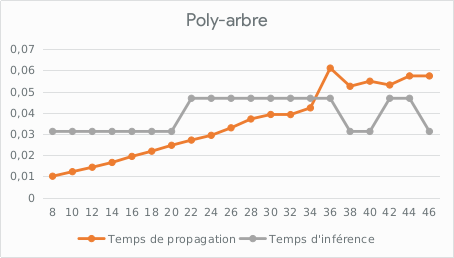
\includegraphics[width=0.75\linewidth]{sheets/poly.png}
	\end{figure}

    \paragraph{Commentaires}:
    Comme nous pouvions nous y attendre, le cas du polygraphe est aisément simple à traiter, surtout que la phase de construction de l'arbre de jonction n'est pas nécessaire, ce qui explique la rapidité de la propagation, l'inférence logique est aussi très performante, mais puisque c'est un exemple simple d'un polyarbre nous ne pouvons pas conclure sur la performance des deux, quoique qu'on peut observer une augmentation quasi-linéaire pour la propagation contre une stabilité de l'inférence.
	
	\subsubsection{Réseau faiblement multi-connecté}
	\paragraph{}
	Dans ce cas, nous considérons le cas d'un graphe multi-connecté, par conséquent, le passage par la construction de l'arbre de jonction
	est nécessaire, cela ralentit consédérablement le temps d'exécution, mais ne devrait pas influencer
	sur le temps de propagation, ce temps dépend surtout de la talle du réseau, les résultats obtenus sont les suivants :

	%LOW
	\begin{table}[H]
	\centering
	\resizebox{\textwidth}{!}{%
	\begin{tabular}{|c|c|c|c|c|}
	\hline
	\textbf{Nombre noeud} & \textbf{Nombre parent} & \textbf{degré de possibilité} & \textbf{Temps de propagation} & \textbf{Temps d'inférence} \\ \hline
	8                     & 5                      & 0.049787                      & 0.0031867                     & 0.046875                   \\ \hline
	16                    & 5                      & 1.67E-05                      & 0.0082458                     & 0.078125                   \\ \hline
	24                    & 5                      & 0.13534                       & 0.015874                      & 0.09375                    \\ \hline
	32                    & 5                      & 0.049787                      & 0.023162                      & 0.10375                    \\ \hline
	40                    & 5                      & 1                             & 0.39958                       & 0.140625                   \\ \hline
	\end{tabular}%
	}
	\end{table}

	\begin{figure}[H]
		\centering
		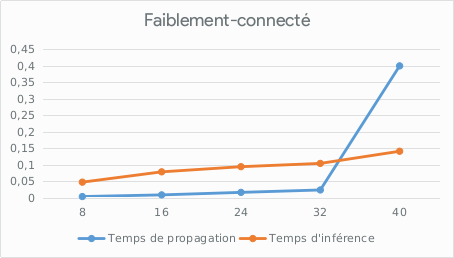
\includegraphics[width=0.75\linewidth]{sheets/weakly.png}
	\end{figure}

	\paragraph{Commentaires}
	On peut remarquer que pour un nombre de noeud petit, le temps de propagation reste très rapide, et cela même comparé au
	temps d'inférence, mais dès qu'on commence à augmenter ce nombre de noeud, une nette amélioration peut être ressentie, elle
	reste encore très peu notable, le passage vers la catégorie suivante pourrait nous donner plus de détails.


	\subsubsection{Réseau moyennement multi-connecté}
	\paragraph{}
	De même que pour la catégorie précédente, mais de façon plus notable, le temps de construction de l'arbre de jonction commence
	à se faire sentir, mais le temps de propagation reste encore à être testé.

	%MEDIUEM
	\begin{table}[H]
	\centering
	\resizebox{\textwidth}{!}{%
	\begin{tabular}{|c|c|c|c|c|}
	\hline
	\textbf{Nombre noeud} & \textbf{Nombre parent} & \textbf{degré de possibilité }& \textbf{Temps de propagation} & \textbf{Temps d'inférence} \\ \hline
	8            & 8             & 0.36788              & 0.0054502            & 0.046875          \\ \hline
	16           & 8             & 0.00091188           & 0.0080397            & 0.0525            \\ \hline
	24           & 8             & 1                    & 0.025212             & 0.078125          \\ \hline
	32           & 8             & 0.049787             & 0.73254              & 0.078125          \\ \hline
	40           & 8             & 0.13534              & 11.451               & 0.109375          \\ \hline
	\end{tabular}%
	}
	\end{table}

	\begin{figure}[H]
		\centering
		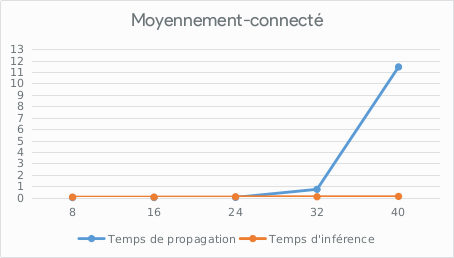
\includegraphics[width=0.75\linewidth]{sheets/medium.png}
	\end{figure}

	\paragraph{Commentaires}
	Ici nous pouvons finalement apprécier la puissance de l'algorithme d'inférence, en effet pour une grand nombre de noeud,
	et une densité dans la distribution des relations entre noeud (40 noeuds, 8 parents) le temps de propagation dépasse les 
	10 secondes(sans compter le temps de construction de l'arbre de jonction), alors que le passage vers la base possibiliste
	et le lancement de l'inférence se fait dans un temps très raisonnable. C'est ainsi un premier indicateur que la représentation
	graphique peut avoir des limite comme nous l'avons anticipé.

	\subsubsection{Réseau fortement multi-connecté}
	\paragraph{}
	Ici nous poussons le bouchon aux limites, en théorie, pour un grand nombre de noeud, la construction de l'arbre de jonction
	ne devrait pas se terminer, soit par cause de time-out ou de dépassement de capacité mémoire (c'est cette dernière que nous
	rencontré durant le test pour les grandes valeurs). Reste a comparé avec les performances de l'inférence logique.


	% HIGH
	\begin{table}[H]
	\centering
	\resizebox{\textwidth}{!}{%
	\begin{tabular}{|c|c|c|c|c|}
	\hline
	\textbf{Nombre noeud} & \textbf{Nombre parent} & \textbf{degré de possibilité} & \textbf{Temps de propagation} & \textbf{Temps d'inférence} \\ \hline
	8                     & 14                     & 0.0067379                     & 0.0027797                     & 0.109375                   \\ \hline
	16                    & 14                     & 0.13534                       & 0.0075522                     & 0.265625                   \\ \hline
	24                    & 14                     & 0.018316                      & 0.37983                       & 0.515625                   \\ \hline
	32                    & 14                     & 0.018316                      & 8.0161                        & 0.3125                     \\ \hline
	40                    & -                      & -                             & -                             & -                          \\ \hline
	\end{tabular}%
	}
	\end{table}

	\begin{figure}[H]
		\centering
		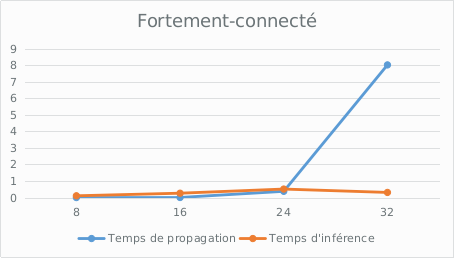
\includegraphics[width=0.75\linewidth]{sheets/strongly.png}
	\end{figure}

	\paragraph{Commentaires}
	Comme anticipé, la propagation graphique montre de grande lacunes, entre le long temps de construction et propagation pour un 
	nombre de noeud égale à 32, et la saturation de la mémoire pour ce même nombre égale à 40, et la vitesse quasi-instantanée 
	d'influencer logique, le choix est vite fait.

	\chapter{Conclusion}
	\paragraph{}
	Au terme de TP, nous avons pu pu appliquer les aspects théoriques vu en cours, afin de mieux apprécier la puissance des
	algorithmes d'inférence(que ce soit en terme logique ou par son équivalent graphique, c.à.d la propagation).
	\par 
	Ce que nous pouvons tirer comme conclusion, est qu dans des cas simples c.à.d (petit nombre de variable et faible dépendance
	entre elles) les deux technique de calculs du degré de possibilité se valent, avec un bonus pour l'inférence logique du point
	de vue régularité(temps de réponses stable). En revanche dans les cas complexes, du moins ceux que nous avons étudié, l'inférence
	à de grand avantages par rapport à son homologue graphique, plusieurs raisons peuvent être données comme la complexité 
	temporelle théorique (Complexité exponentielle contre Complexité logarithmique).
	\par 
	En revanche nous n'avons pas pu effectuer d'autre testes plus poussé pour connaître les limites de l'inférence logique, de ce 
	fait décider de quelle méthode est préférable à une autre serait trop prématuré, mais dans les cas que nous avons vu jusqu'à 
	maintenant, l'inférence remporte le match haut la main.




\end{document}